\section{Results}
\begin{figure}[H]
%\begin{align*}
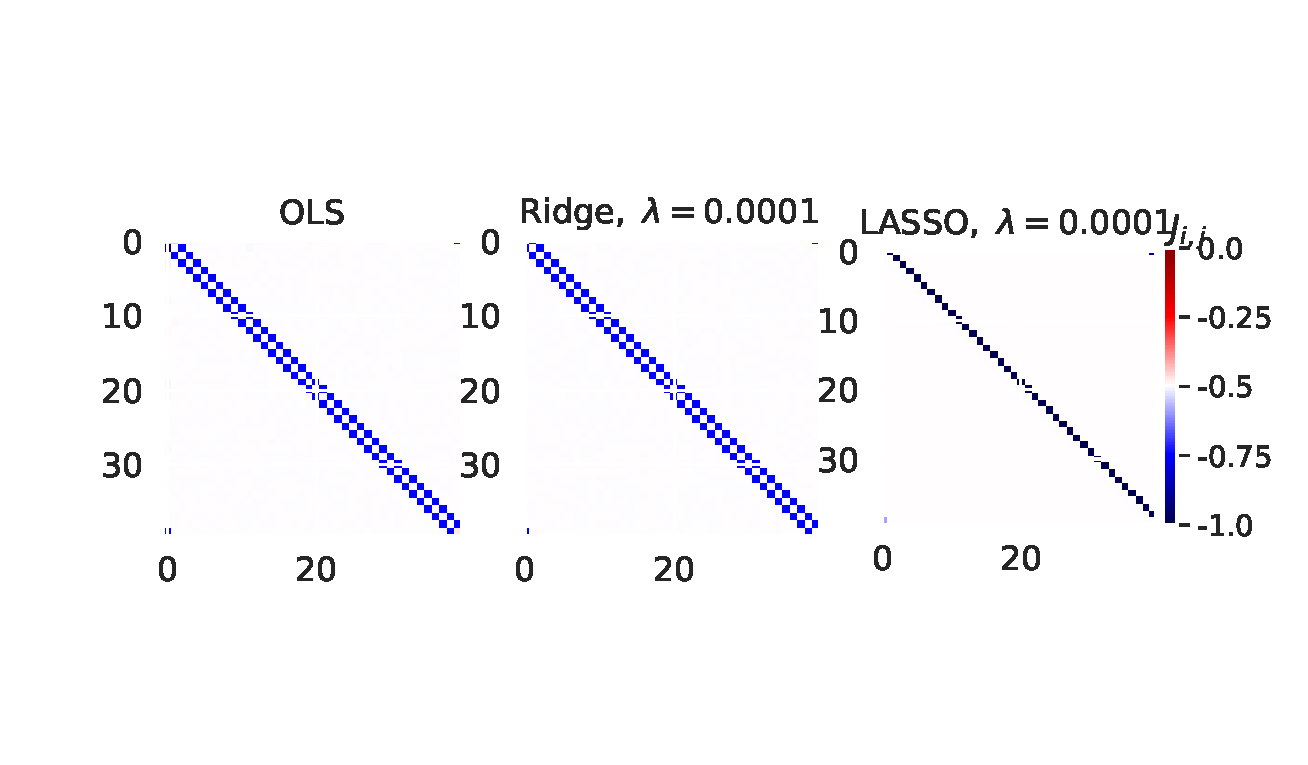
\includegraphics[width = 0.7\paperwidth]{figures/regression_mehta_1.pdf}
\end{figure}
%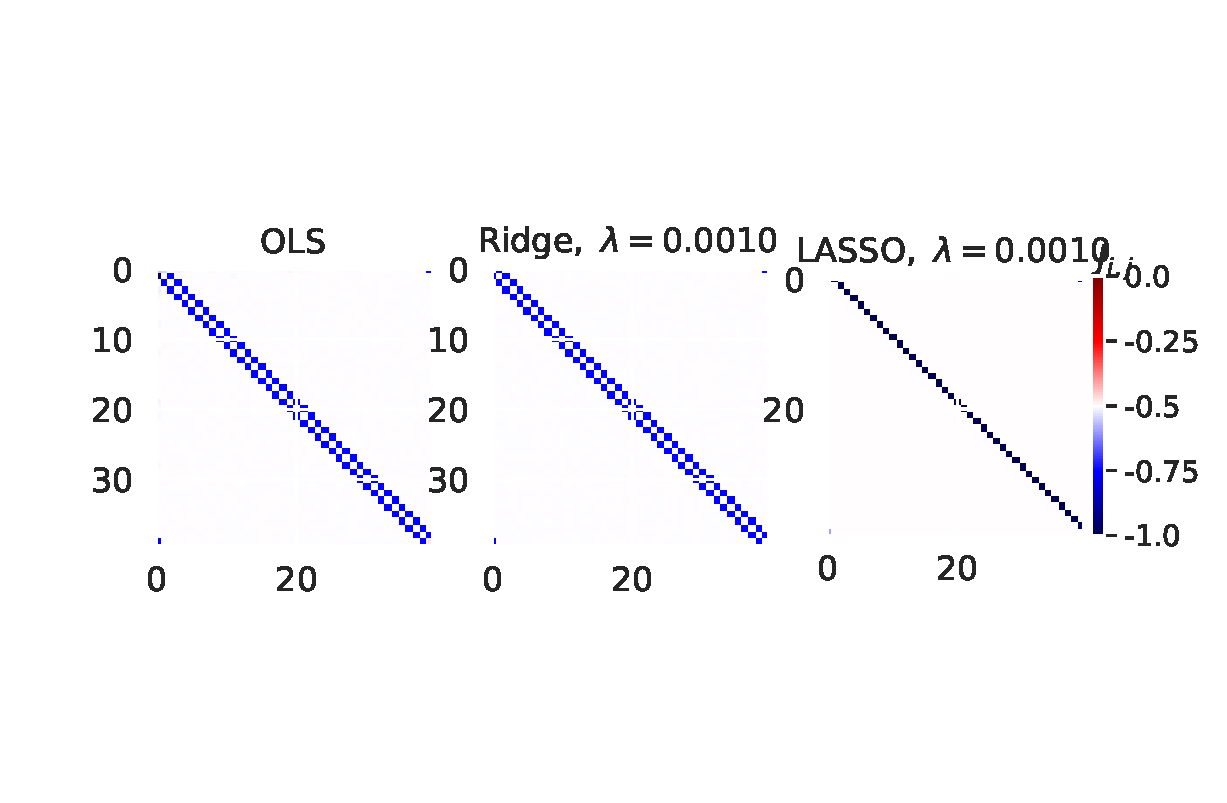
\includegraphics[width = 0.8\paperwidth]{figures/regression_mehta_2.pdf} \\
\begin{figure}[H]
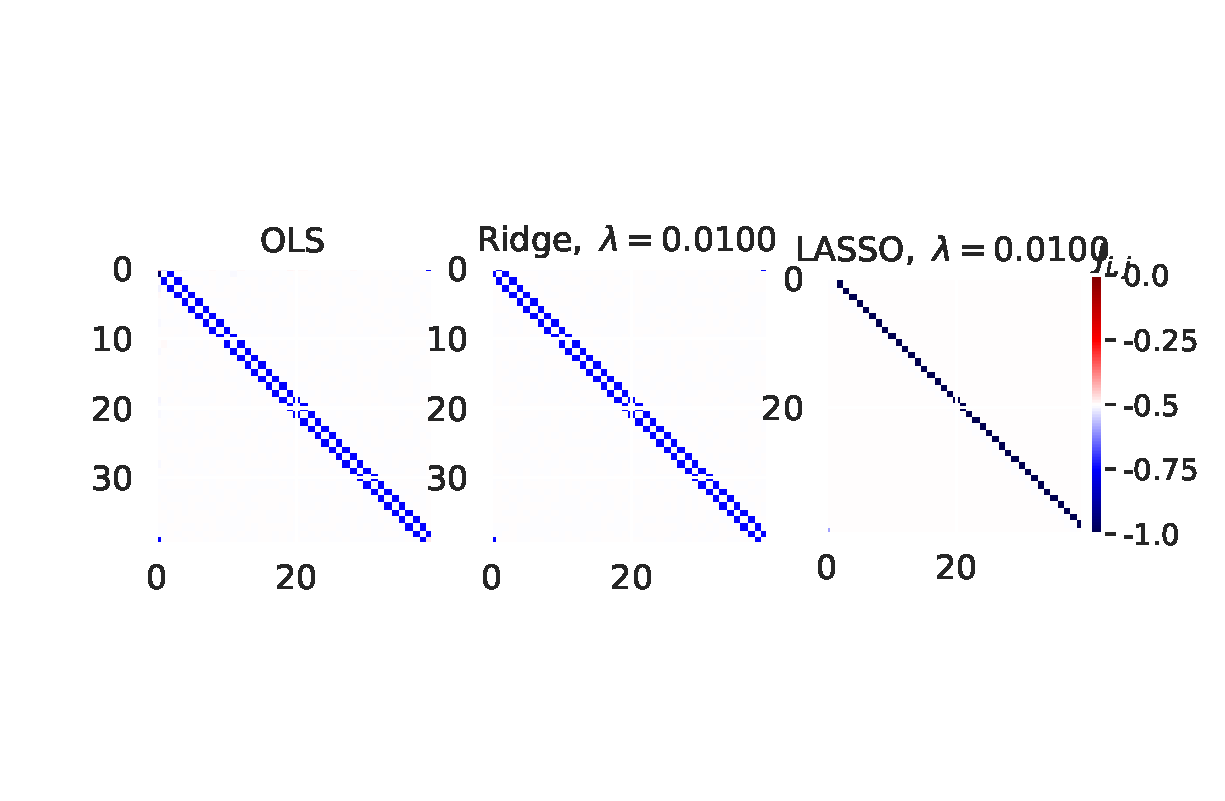
\includegraphics[width = 0.7\paperwidth]{figures/regression_mehta_3.pdf}\\
\end{figure}
%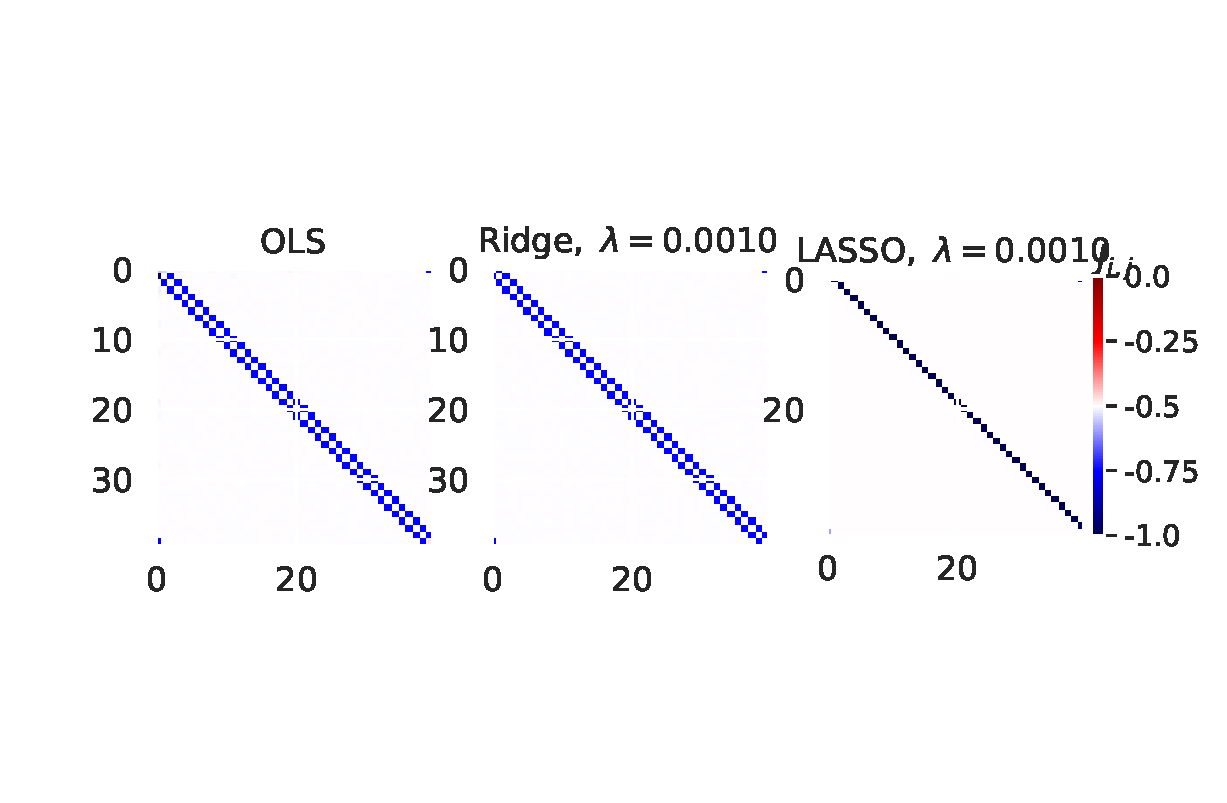
\includegraphics[width = 0.8\paperwidth]{figures/regression_mehta_2.pdf} \\ 
%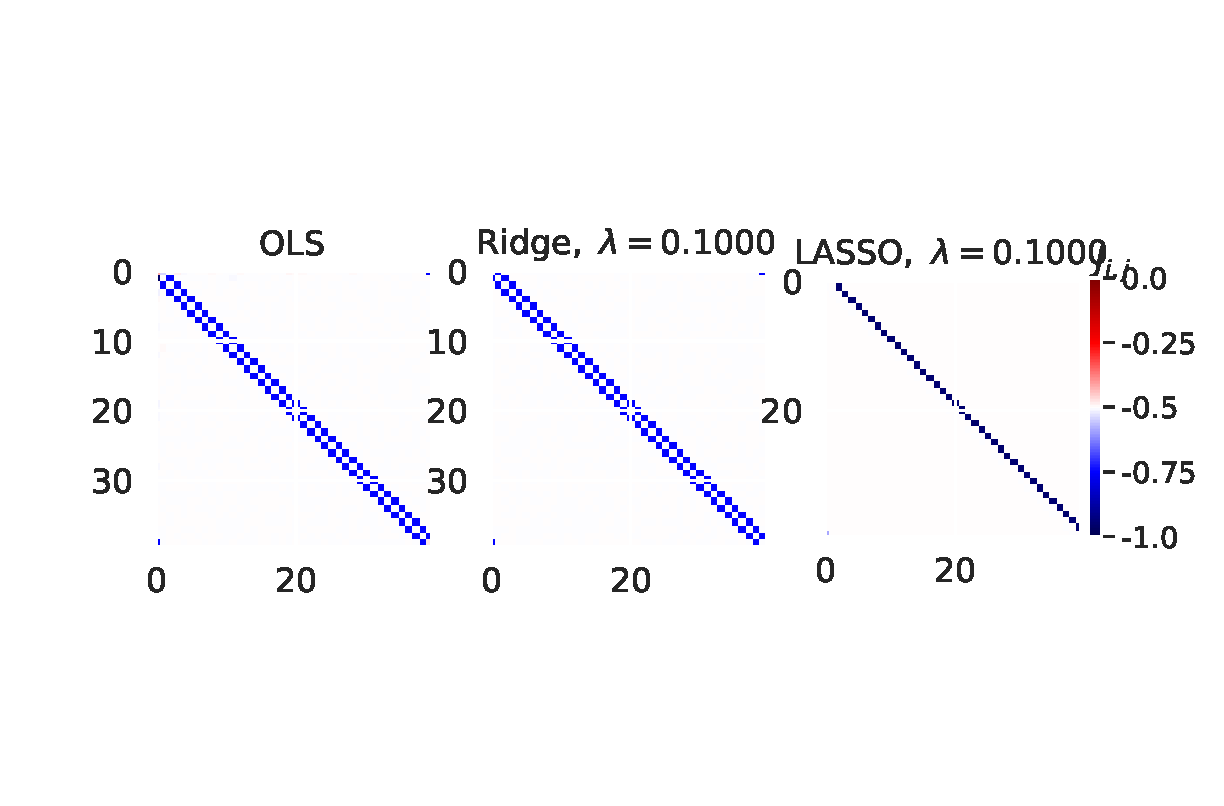
\includegraphics[width = 0.8\paperwidth]{figures/regression_mehta_4.pdf} \\
\begin{figure}[H]
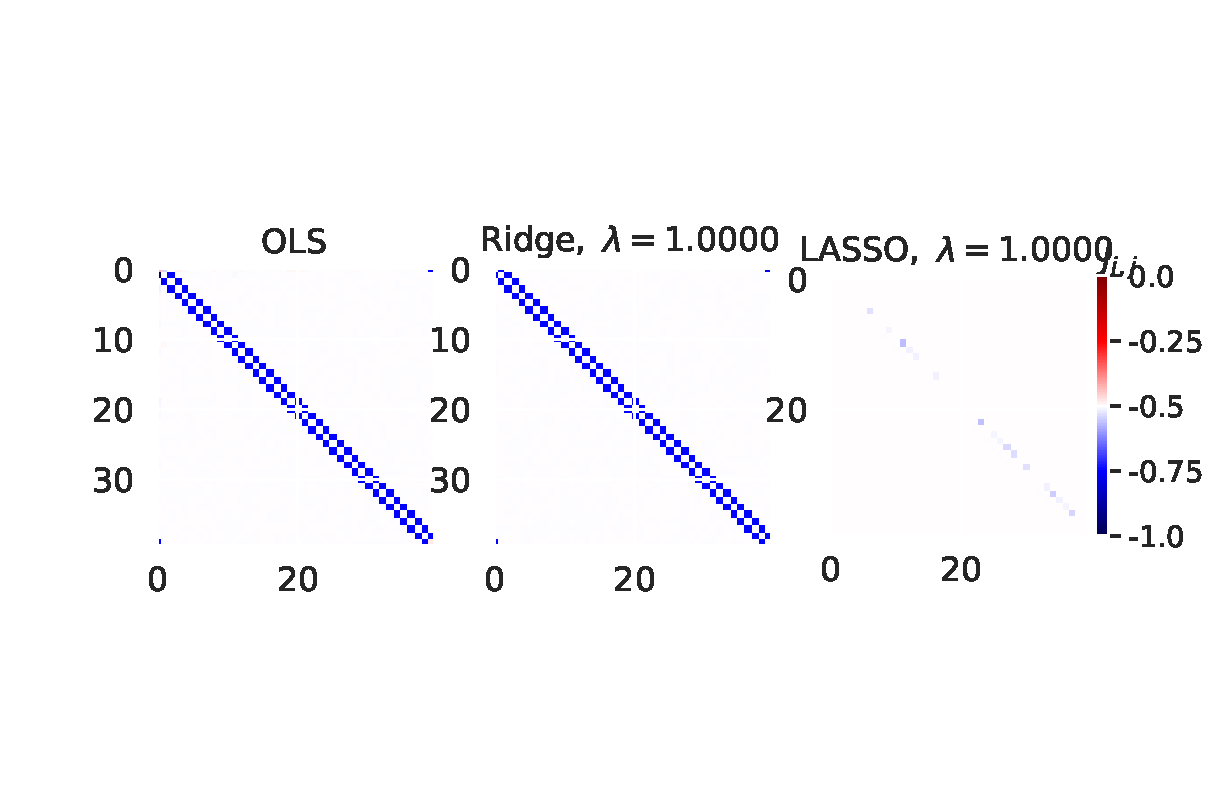
\includegraphics[width = 0.6\paperwidth]{figures/regression_mehta_5.pdf} \\
\end{figure}
%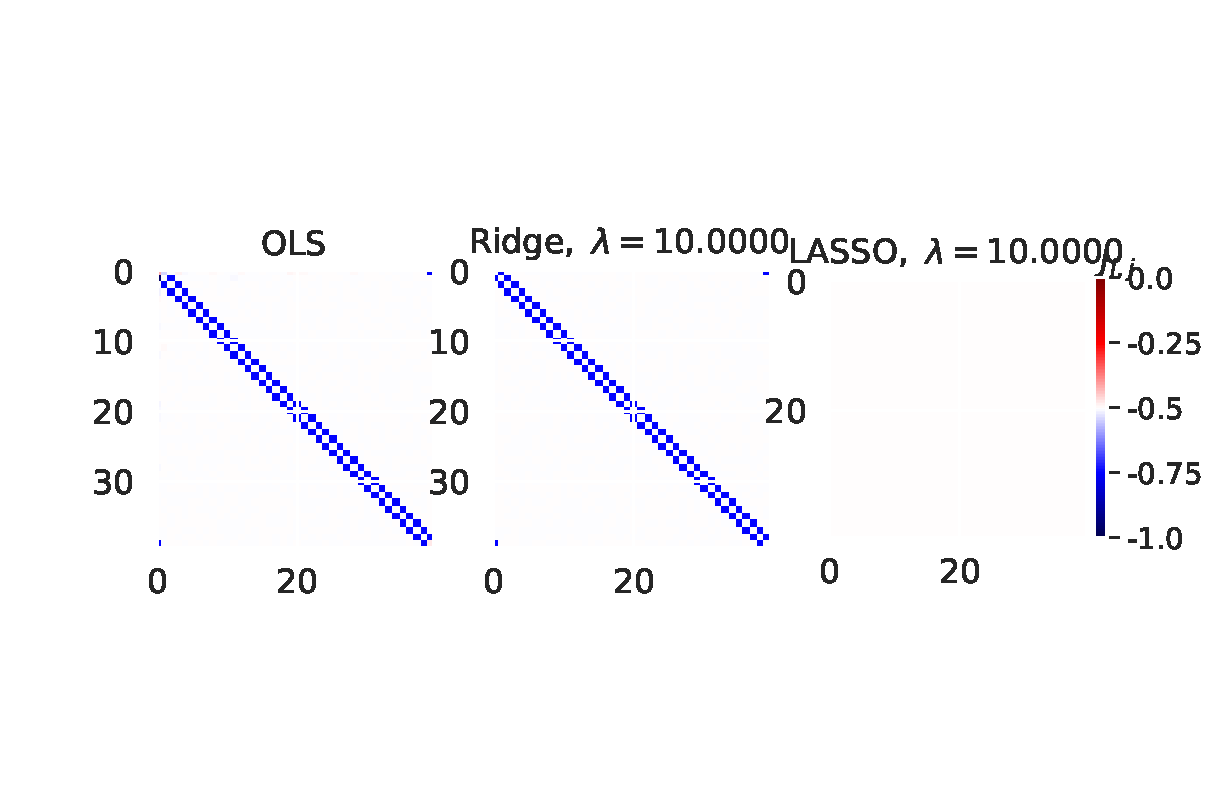
\includegraphics[width = 0.8\paperwidth]{figures/regression_mehta_6.pdf} \\
%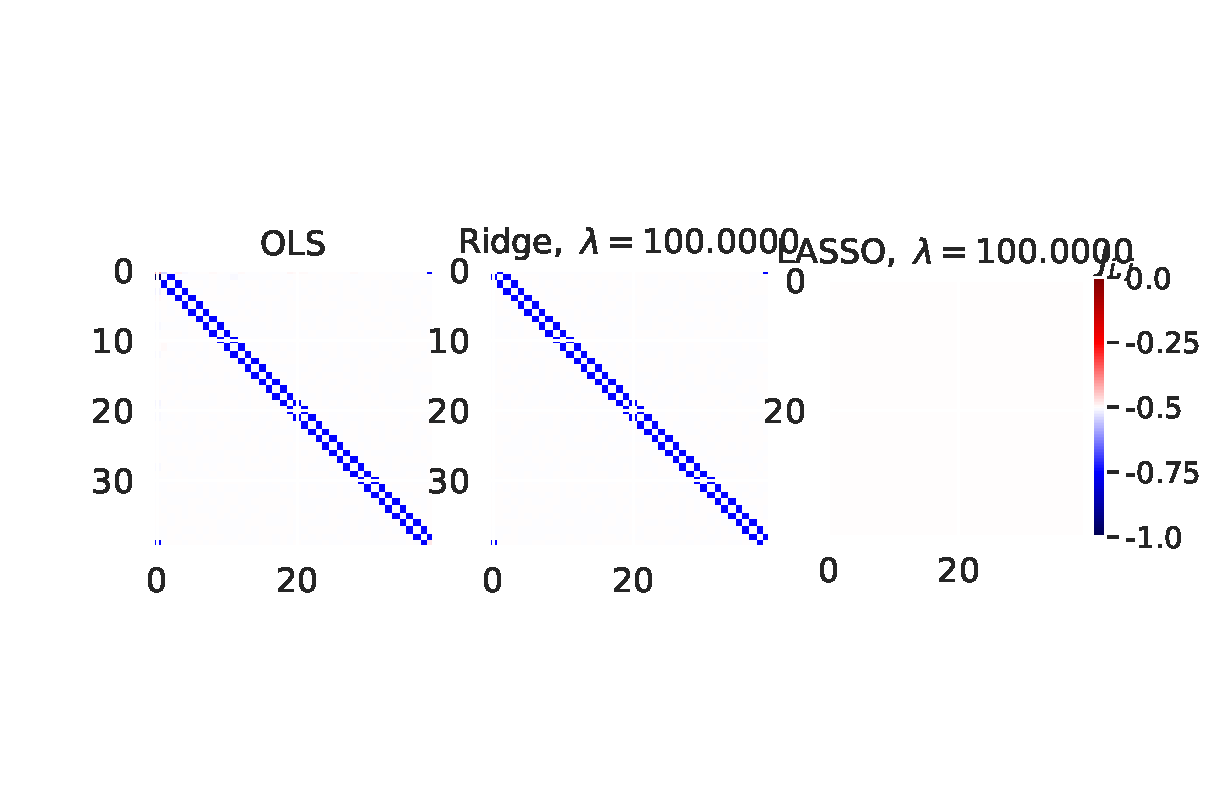
\includegraphics[width = 0.8\paperwidth]{figures/regression_mehta_7.pdf} \\
%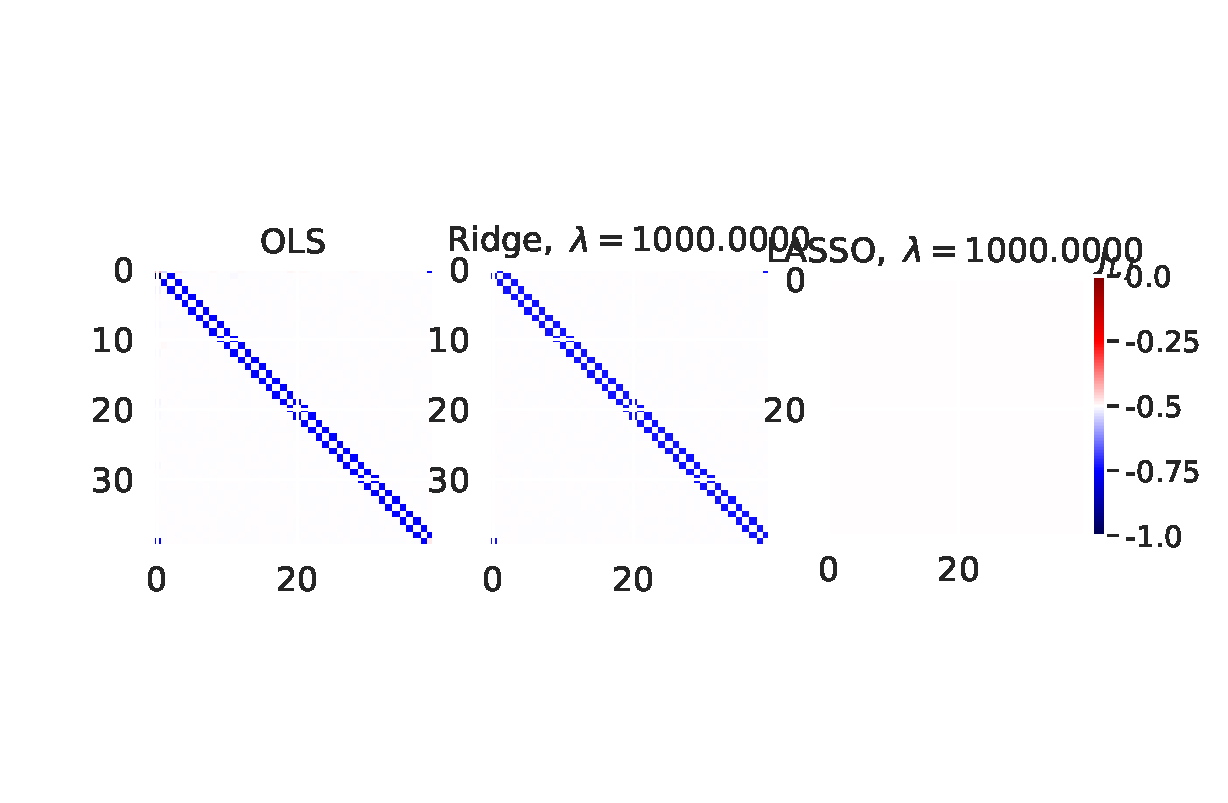
\includegraphics[width = 0.8\paperwidth]{figures/regression_mehta_8.pdf} \\
\begin{figure}[H]
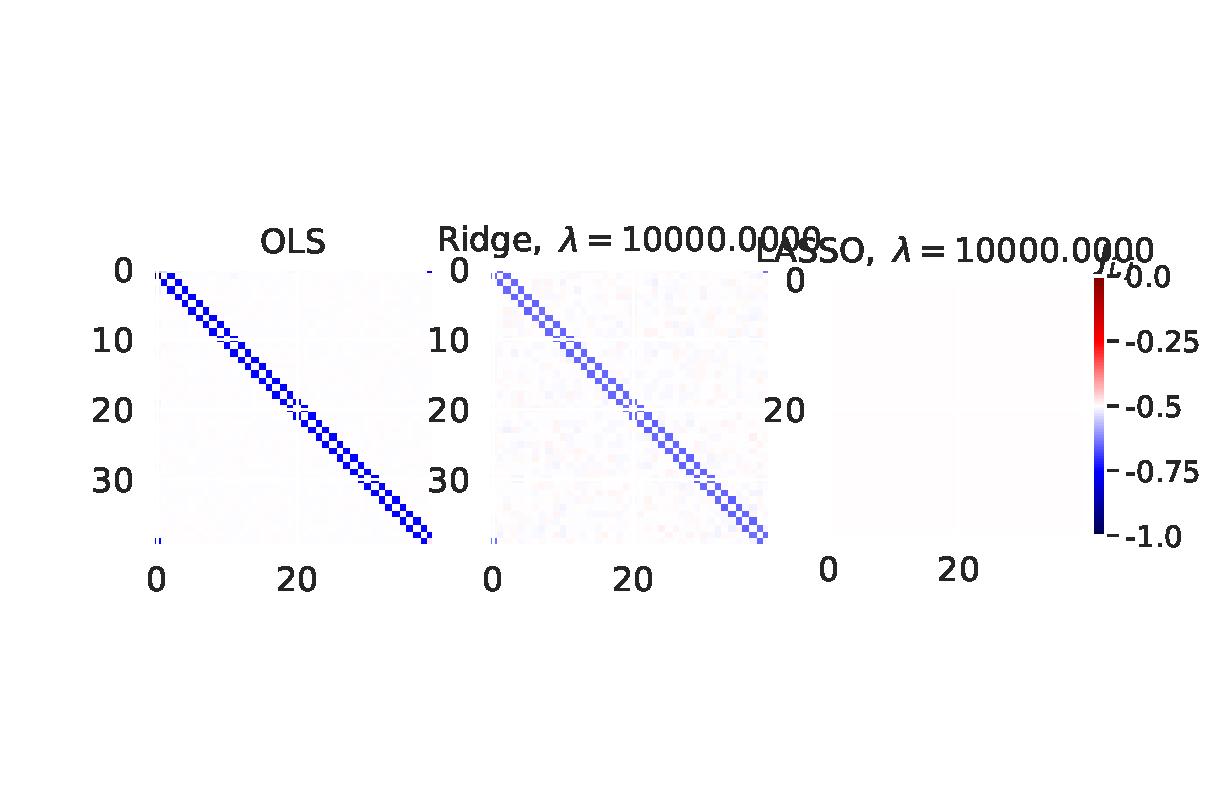
\includegraphics[width = 0.6\paperwidth]{figures/regression_mehta_9.pdf} \\
%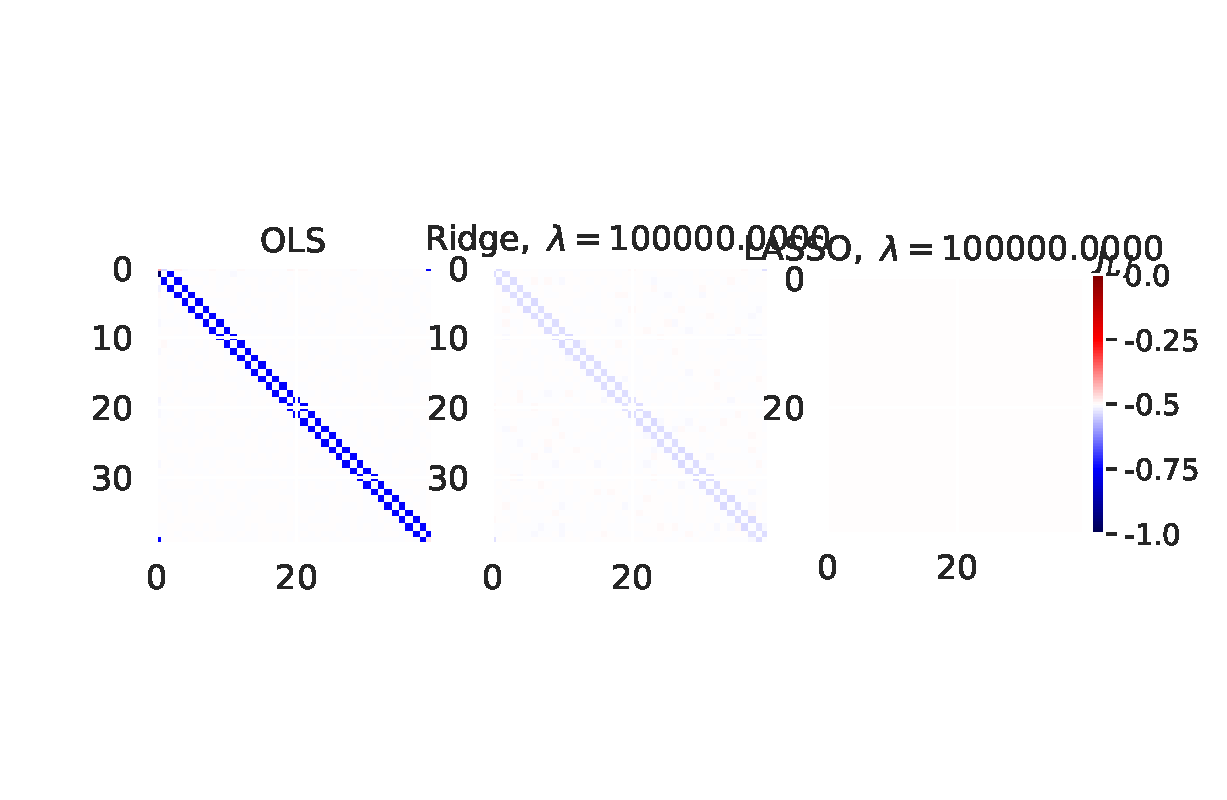
\includegraphics[width = 0.8\paperwidth]{figures/regression_mehta_10.pdf}
%\end{align*}
\caption{Ising model plots for selected regularization parameters $\lambda$, generated based on our regression models.
	 } 
\label{fig:regression-mehta}
\end{figure}

\begin{figure}[H]
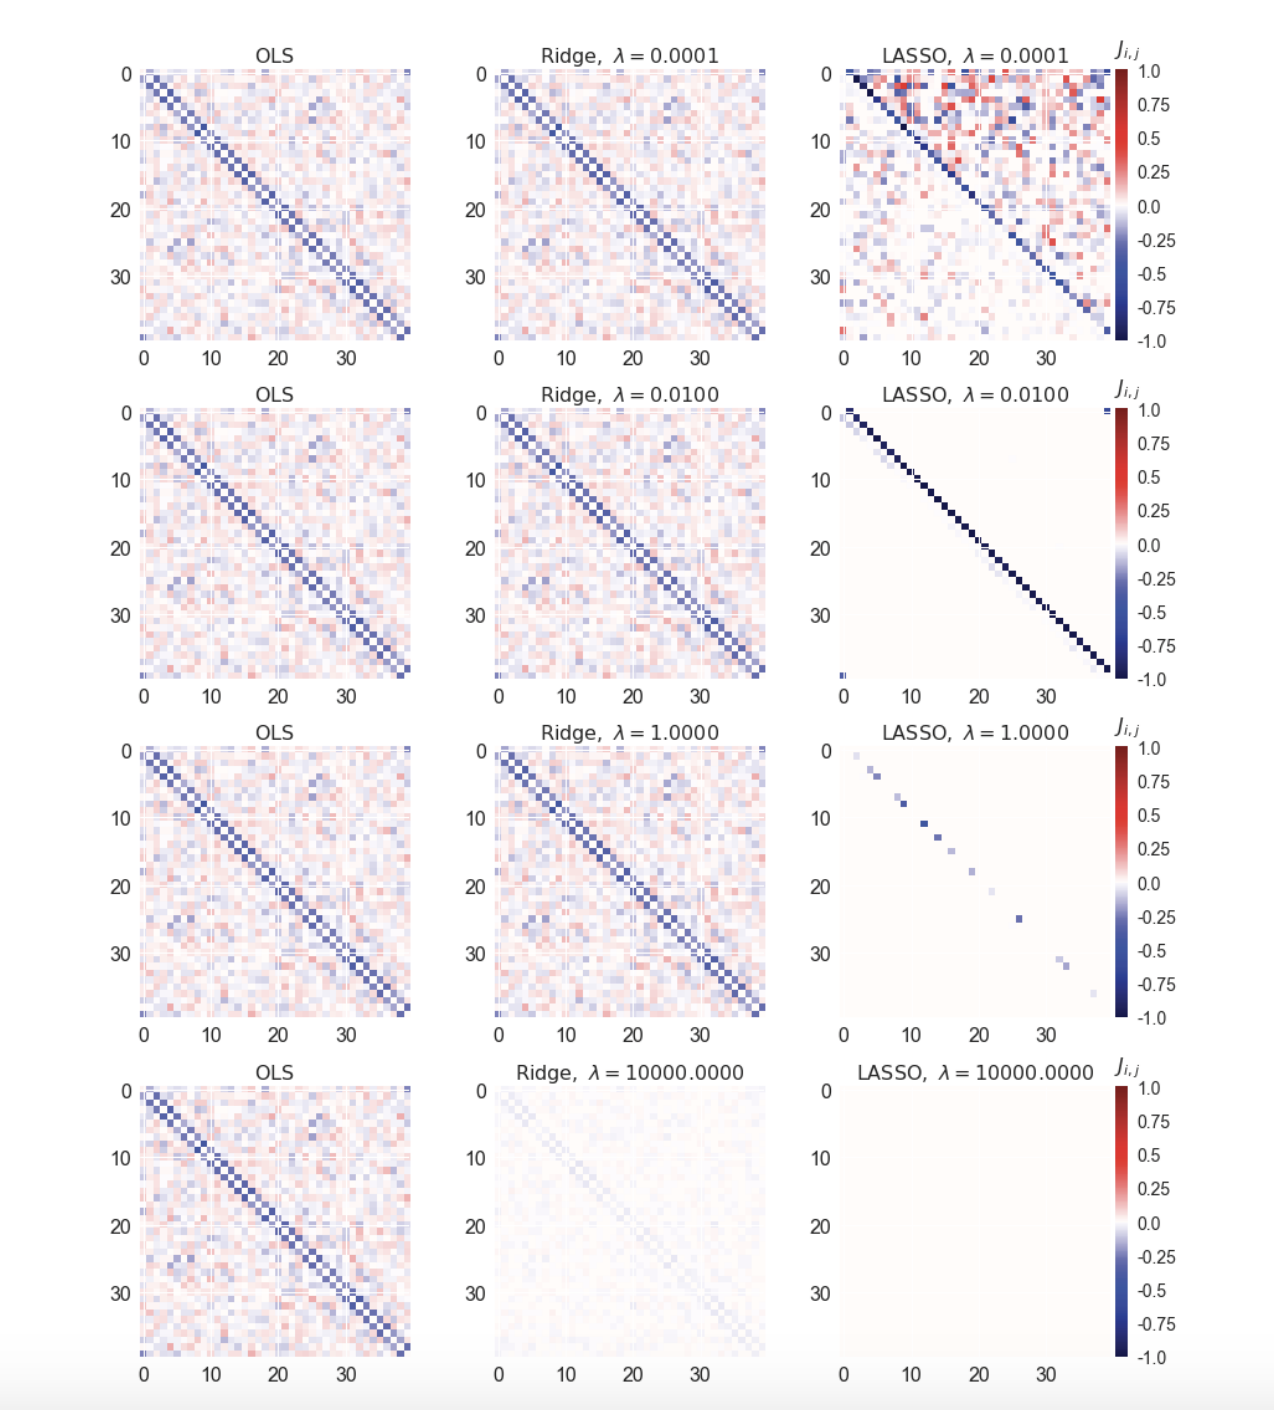
\includegraphics[width = 0.7\paperwidth]{figures/Regression_metha_article.png} 
\caption{Figures from article ~\cite{HighBias} shows similarities to the ones generated by our regression models.} 
\label{fig:regression-mehta}
\end{figure}

Based on the figures above, we see that the figure in article ~\cite{HighBias} 
is similar to out own figures. The figure in the article. Our figures
shows less noice, and some other small differences,  but we see that the tendencies are the same. 

\begin{figure}[H]
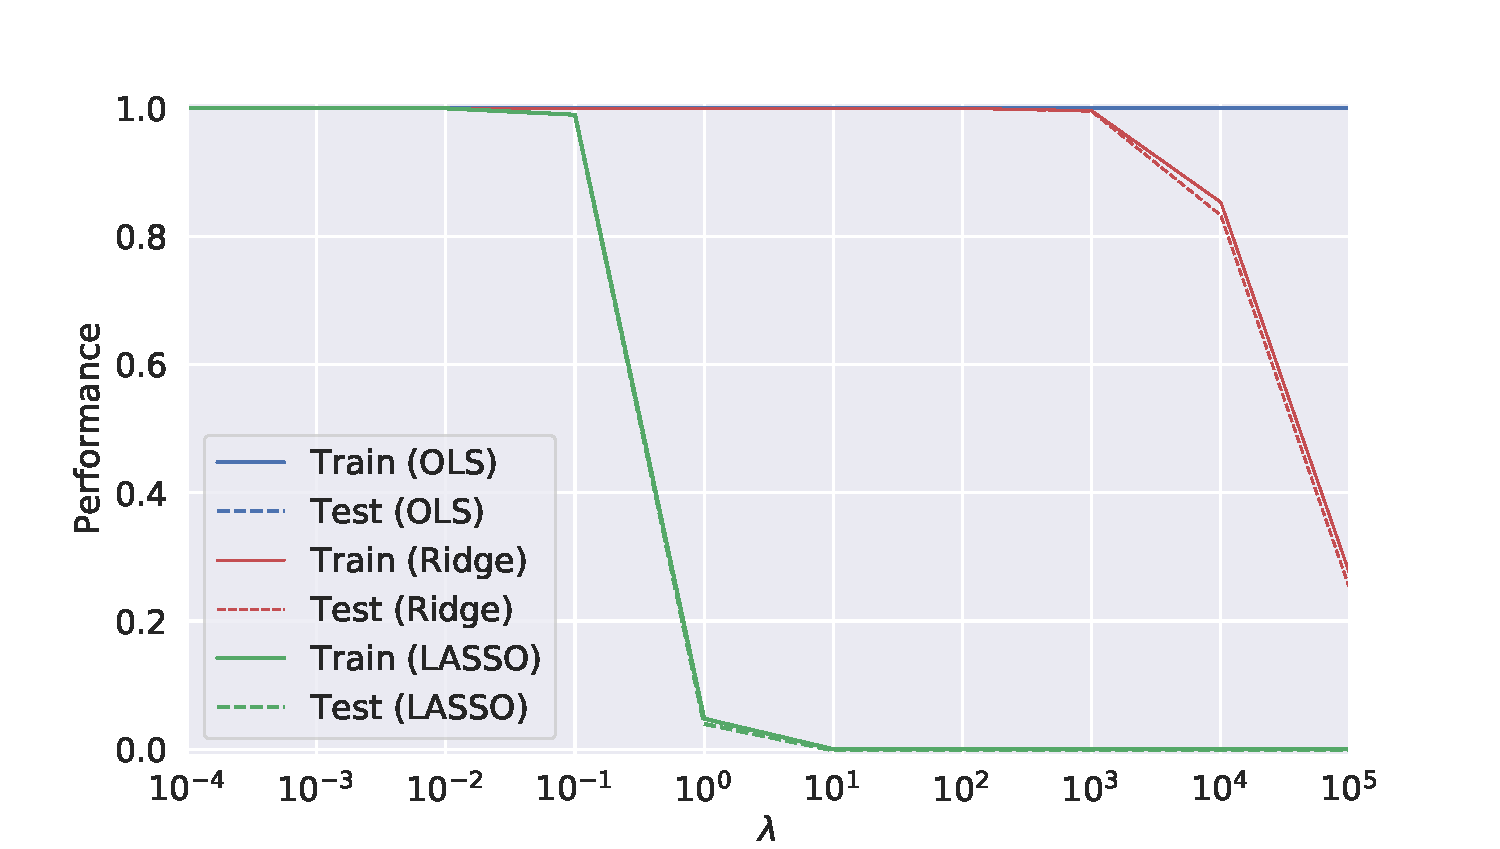
\includegraphics[width = 0.8\paperwidth]{figures/regression_r2.pdf}
    \caption{R2 score performance of the linear regression models as a function of
	     regression parameter $\lambda$.}
\label{fig:regression-r2}
\end{figure}
Figure \ref{fig:regression-r2} show how the R2 score varies between models. It's important
to note that the $\lambda$ for Ridge regression, and $\alpha$ for Lasso regression have
the same value, but they affect the models on different orders of magnitude, and must be
treated somewhat separately. Even so, we can see that the training and test set R2-scores
follow eachother closely.
\begin{figure}[H]
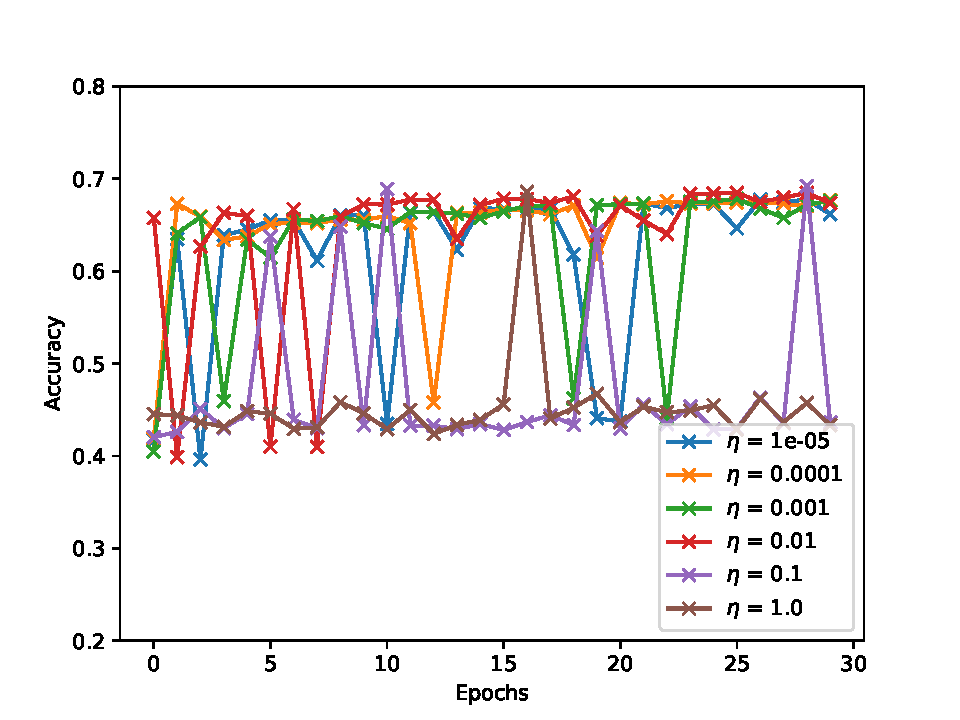
\includegraphics[width = 0.8\paperwidth]{figures/logistic_eta.pdf}
    \caption{Accuracies for a selection of learning rates $\eta$ as a function of epochs. 
    30 epochs, batch size $= 100$, and momentum parameter $\gamma = 0.01$. The accuracy
    values are measured on the test set.
    The ratio of amount of training data to test data is $0.8$.}
\label{fig:logistic-eta}
\end{figure}
Figure \ref{fig:logistic-eta} show the results for learning rate $\eta$ comparison when applying
our logistic regression model on the Ising Model data. For some $\eta$ the model quickly rises
to an approximate highest value, but jumps back down to the equivalent of guessing from time
to time. When approaching 30 epochs and more, this behaviour seems to diminish somewhat, and
overall the etas that produce the best results ($10^{-5} - 10^{-2}$) have most of their values
in the higher points.
\begin{table}[H]
\center
\begin{tabular}{l|c|c|c}
$\eta$ & Training & Test & Critical  \\
\hline
$10^{-5}$ & $0.718$ & $0.680$ & $0.616$ \\
$10^{-4}$ & $0.723$ & $0.683$ & $0.624$ \\
$10^{-3}$ & $0.723$ & $0.685$ & $0.628$ \\
$10^{-2}$ & $0.712$ & $0.672$ & $0.604$ \\
$10^{-1}$ & $0.462$ & $0.430$ & $0.460$ \\
$1$    & $0.465$ & $0.446$ & $0.480$
\end{tabular}
    \caption{Accuracies for a selection of learning rates $\eta$ after 
    30 epochs. Batch size $= 100$, and momentum parameter $\gamma = 0.01$.
    The ratio of amount of training data to test data is $0.8$}
    \label{tab:logistic-critical}
\end{table}
In table \ref{tab:logistic-critical} the accuracy on data containing critical states
is included. Due to the varying nature our logistic model, a solution in which the weights
producing the best fit on test data are stored was developed. The accuracies for the critical
states are thus not necessarily produced with weights as they are after 30 epochs.


